% Generated by code/needham.py -- do not edit by hand.
\definecolor{qocA}{rgb}{0.00,0.45,0.70}
\definecolor{qocB}{rgb}{0.90,0.60,0.00}
\definecolor{qocC}{rgb}{0.00,0.62,0.45}
\definecolor{qocD}{rgb}{0.80,0.40,0.00}
\definecolor{qocE}{rgb}{0.80,0.60,0.70}
\definecolor{qocF}{rgb}{0.35,0.70,0.90}
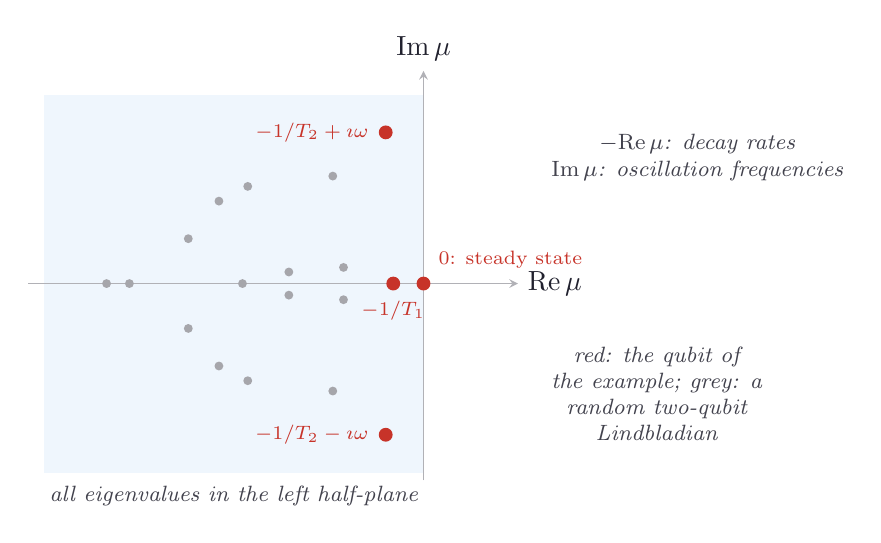
\begin{tikzpicture}[ink/.style={line width=0.9pt, ndInk}, faint/.style={line width=0.4pt, ndInk!35}, dashedink/.style={line width=0.5pt, ndInk!55, dash pattern=on 2.5pt off 2pt}, vec/.style={->, >=stealth, line width=1.2pt}, note/.style={font=\footnotesize\itshape, text=ndInk!85, align=center}, pointer/.style={->, >=stealth, line width=0.4pt, ndInk!60, shorten >=2pt, shorten <=1pt}, dot/.style={circle, fill=ndInk, inner sep=0pt, minimum size=3.4pt}, wash/.style={fill=ndSky, fill opacity=0.55}, every node/.style={text=ndInk}]
\definecolor{ndInk}{rgb}{0.13,0.13,0.18}
\definecolor{ndPaper}{rgb}{0.99,0.96,0.88}
\definecolor{ndSky}{rgb}{0.84,0.91,0.98}
\definecolor{ndRose}{rgb}{0.98,0.86,0.84}
\definecolor{ndBlue}{rgb}{0.13,0.36,0.66}
\definecolor{ndRed}{rgb}{0.78,0.20,0.16}
\definecolor{ndGold}{rgb}{0.88,0.62,0.10}
\definecolor{ndGreen}{rgb}{0.18,0.52,0.30}
\fill[ndSky, fill opacity=0.4] (-4.82,-2.40) rectangle (0,2.40);
\draw[faint, ->, >=stealth] (-5.02,0) -- (1.20,0) node[right, text=ndInk] {$\mathrm{Re}\,\mu$};
\draw[faint, ->, >=stealth] (0,-2.50) -- (0,2.70) node[above, text=ndInk] {$\mathrm{Im}\,\mu$};
\fill[ndInk!40] (0.000,0.000) circle (1.6pt);
\fill[ndInk!40] (-1.152,1.365) circle (1.6pt);
\fill[ndInk!40] (-1.152,-1.365) circle (1.6pt);
\fill[ndInk!40] (-4.025,0.000) circle (1.6pt);
\fill[ndInk!40] (-3.735,-0.000) circle (1.6pt);
\fill[ndInk!40] (-2.232,1.234) circle (1.6pt);
\fill[ndInk!40] (-2.598,1.047) circle (1.6pt);
\fill[ndInk!40] (-2.987,0.570) circle (1.6pt);
\fill[ndInk!40] (-2.232,-1.234) circle (1.6pt);
\fill[ndInk!40] (-2.598,-1.047) circle (1.6pt);
\fill[ndInk!40] (-2.987,-0.570) circle (1.6pt);
\fill[ndInk!40] (-1.016,0.205) circle (1.6pt);
\fill[ndInk!40] (-1.016,-0.205) circle (1.6pt);
\fill[ndInk!40] (-2.299,0.000) circle (1.6pt);
\fill[ndInk!40] (-1.710,0.147) circle (1.6pt);
\fill[ndInk!40] (-1.710,-0.147) circle (1.6pt);
\node[dot, fill=ndRed, minimum size=5pt, label={[font=\scriptsize, text=ndRed]above right:$0$: steady state}] at (0.000,0.000) {};
\node[dot, fill=ndRed, minimum size=5pt, label={[font=\scriptsize, text=ndRed]below:$-1/T_1$}] at (-0.384,0.000) {};
\node[dot, fill=ndRed, minimum size=5pt, label={[font=\scriptsize, text=ndRed]left:$-1/T_2+\imath\omega$}] at (-0.480,1.920) {};
\node[dot, fill=ndRed, minimum size=5pt, label={[font=\scriptsize, text=ndRed]left:$-1/T_2-\imath\omega$}] at (-0.480,-1.920) {};
\node[note, anchor=west] at (1.50,1.60) {$-\mathrm{Re}\,\mu$: decay rates\\ $\mathrm{Im}\,\mu$: oscillation frequencies};
\node[note, anchor=west] at (1.50,-1.40) {red: the qubit of\\ the example; grey: a\\ random two-qubit\\ Lindbladian};
\node[note, anchor=north] at (-2.41,-2.45) {all eigenvalues in the left half-plane};
\end{tikzpicture}
